\chapter{Model Decomposition}

In order to represent the internal structure of a model, we decomposed 
the base model into multiple cells covering the whole volume of the object.
A core part of this project has been focused on the model decomposition,
as well as on algorithms to produce and improve said decomposition. In this
section of the thesis we are going to take a deep dive into the basic method
taken from \cite{10.2312:ceig.20241139} and all the improvements we added.

\section{Base Method Overview}

As statet eariler, the main idea of the decomposition process is to divide
the original model into multiple shards that are connected with bonds (that 
we call links). In order to generate the fragments of the models, which 
will be called cells from now on, a voronoi tessellation is used, as they 
produce a more natural rocky appearance than other possible decompositions like 
voxelizations or tetrahedalizations. The process of generating is further 
divided in multiple steps: \textbf{Point Extraction}, \textbf{Voronoi Cells 
Generation} and \textbf{Links Generation}. Additionally we also experimented 
with multi-resolution decompositions, where one cell on the lower resolution 
contains multiple cells on the higher resolution level, this adds an additional
step that consists on creating the lower resolution levels from the higher one.


\vspace{10pt}

In the original project, they divided the decomposition process in different 
steps, as it can be seen on \ref{fig:Decomposition_diagram}, due to some changes
in the method we changed a the steps a little. Despite that, the main outline 
of the process is similar and our changes reside in the specific steps. 
 

\begin{figure}
    \centering
    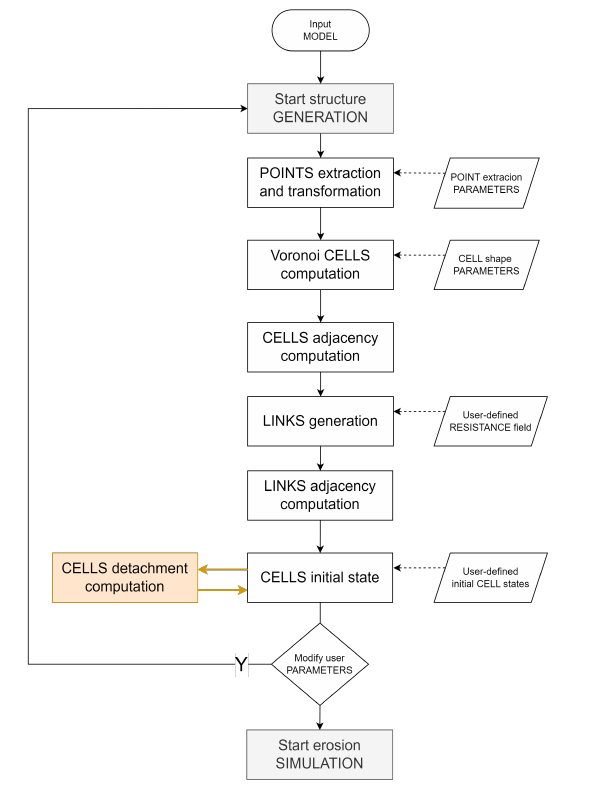
\includegraphics[scale=0.39]{Decomposition/BaseDecomposition.png}
    \caption{Diagram of the original method. Taken from \cite{mateos_arlanzon_2023}}
    \label{fig:Decomposition_diagram}
\end{figure}

\section{Point and Cell Generation}
Remember that voronoi tessellations are partitions of a model into 
different regions, where, given a set of centroids $C = \{c_1, c_2, \hdots , c_n\}$,
the set of regions $\mathbf{R} = \{R_1, R_2, \hdots, R_n\}$ is defined by: 
\begin{equation}
R_i = \{p \in \Omega | \forall c_j \in C, \; \;  d(p, c_i) \leq d(p, c_j)\}
\end{equation}
Where $\Omega \in \mathbb{R}^3$ is the domain of our model, $d$ represents 
the euclidean distance and $c_i$ is the centroid of region $i$.

\vspace{10pt}

This definition implies that the only thing we need in order to construct a 
voronoi tessellation is a set of centroids that will define our regions, then the 
regions will become our cells defined by the planes that form their boundaries. 
The number of centroids chosen and their positions heavily affect the result
of the tessellation, so the sampling method that we decide to implement will be 
highly relevant for the end result. In addition to the sampling, one more
thing that we will need to take into account is the fact that the regions
that lie on the boundary of the region will be technically unbounded and 
we will have to manually add walls to cut them so they do not leave the 
boundary of the original model.
 
\subsection{Cell Generation} \label{sec:cellGen}

The first step of the voronoi tessellation would be to sample the points 
that we will use as centroids of our cells. Despite that, we think it is 
better to first explain the process of constructing the cells from the 
points, as we took it into account when designing our sampling.

\vspace{10pt}

In order to construct the cells from the centroids we offload the computation
to the library Voro++ \cite{osti_code-54674}, which given a set of points 
and a boundary (with restrictions on the boundary that will be discussed 
in the future) gives us a set of polyhedra representing the different voronoi 
cells. Even if this part of the computation is offloaded to another library 
it is important to know about the process of construction of one voronoi cell.

\vspace{10pt}

Given a pair of centroids $c_i$ and $c_j$, the whole region is divided into 
two half-spaces: $H_{ij}$, where points are closer to $c_i$ than $c_j$; 
and $H_{ji}$, for points closer to $c_j$. More formally we can define $H_{ij}$
the following way: 

\begin{equation}
    H_{ij} = \{p \in \Omega | d(p,c_i) \leq d(p,c_j)\}
\end{equation}

Every point in $R_i$ is closer to $c_i$ than any other centroid $c_k$, so 
it follows that it also has to be in $H_{ik}$ for every $k \neq i$. Conversly,
if we have a point $p \in \Omega$ in $H_{ik}$ for every $k \neq i$, it follows that 
$p \in R_i$. This fact allows us to define the voronoi cell $R_i$ as the 
intersection of a set of hall-spaces:

\begin{equation}
    R_i = \bigcap_{j = 1}^n H_{ij}
\end{equation}

Each half-space is defined by the plane that is equidistant from both centroids,
so this converts the problem of creating a voronoi cell into computing the 
intersection of multiple planes. Keep in mind that $H_{ii}$ would define 
all the domain, since every point is at the same distance from $c_i$ and 
$c_i$, so it does not have any effect adding it to the intersection. A 
nice visual demonstration of the construction of a voronoi cell from 
the intersection of half-spaces is shown in figure \ref{fig:voronoiConstruction}

\begin{figure}
    \centering 
    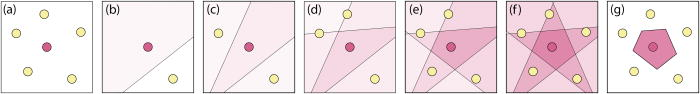
\includegraphics[scale=0.65]{Decomposition/voronoiConstruction.png}
    \caption{Process of construction of a voronoi cell from the intersection
    of half-spaces. figures (b) to (f) show the process of cutting the space 
    into multiple half-spaces, one half-space at a time. Figure taken from 
    \cite{10.1119/5.0087591}}
    \label{fig:voronoiConstruction}
\end{figure}

\vspace{10pt}

To end this section about constructing cells it is important to keep in 
mind that a pair of centroids define a plane where every point on the plane 
is equidistant from both centroids. Let us define this plane more formally, 
as we are going to use it later:

\begin{equation}
    P_{ij}  = P_{ji} = \{p \in \Omega | d(p,c_i) = d(p, c_j)\}
\end{equation}
\subsection{Point Sampling}
The first part of the method will be to sample multiple points inside 
the model to construct a voronoi decomposition. In this thesis, and 
unlike in the base method presented by \cite{mateos_arlanzon_2023}, we 
are using DEMs to represent and load our terrains, so we are going to make 
use of that. 

\vspace{10pt}

A heightfield $\mathcal{H}$ is basically a 2D grid were each
value $h_{ij}$ of the grid represents the height at one cell $(i,j)$ of the gird,
we can then use the points of the grid to obtain the elevation on a continuos domain 
using interpolation. Because we already have a defined grid, we can use 
it to implement our sampling. The main idea is to make use of the 2D grid 
and extend it to a 3D grid by setting a number of vertical samples (which 
will be a user-difine parameter) and then sample one point for each element 
of the grid, as long as the point lies inside the terrain (the 3D grid 
will represent the bounding box of the terrain, so not every voxel will be 
inside it). 

\vspace{10pt}

Now that we have a way to uniformly sample points inside the model, we can 
extend it and break the regularity a little bit by shifting each point by a 
certain quantity. Considering each point to initially be sampled at the 
center of its grid cell, we are going to shift each point by \textit{strictly}
less than half the cell size in a random direction, this way be will 
obtain a sampling in between complete random sampling (white noise) and 
a completly regular sampling, where we guarantee each point to not be to 
close or to far to another. Specifically, from each grid cell center $c_{ijk}$
we create our sample $c_{ijk}'$ using the following equation:

\begin{equation}
    c_{ijk}' = c_{ijk} + \begin{bmatrix} r_xs_x \\ r_ys_y \\ r_zs_z \end{bmatrix}
\end{equation}

Where $s_x$, $s_y$ and $s_z$ are the cell sizes on each direction (we can have 
rectangular cells) and $r_x$, $r_y$ and $r_z$ are three different scalars sampled 
uniformly at random such as $-\frac{1}{2} < -m \leq r_k \leq m < \frac{1}{2}$, where 
$m$ denotes the maximum ammount of shifting allowed and $k \in \{x,y,z\}$. If $m$ 
was $\frac{1}{2}$ then samples will be allowed to lie on the boundary of the 
grid cell, which could result in two samples being at the same place, that is 
why we set $m$ to be \textit{strictly} smaller than $\frac{1}{2}$. 

\vspace{10pt}

Moreover, we can bound the distance between two arbitrary points in terms 
of $m$ and the cell sizes $s_k$. Suppose $s_x$ is the smaller size, 
then the minimum posible distance between two samples $c_{i,j,k}$ 
and $c_{i + 1,j,k}'$ appears when $c_{i,j,k}' = (x + m s_x, y + \alpha s_y, z + \beta s_z)$ 
and $c_{i + 1,j,k}' = (x + s_x - m s_x, y + \alpha s_y, z + \beta s_z)$, so the distance 
is:

\begin{equation}
d(c_{ijk}', c_{i + 1,j,k}') = ||c_{i + 1,jk}' - c_{ijk}'|| = ||(s_x - 2ms_x, 0, 0)|| = s_x(1 - 2m)
\end{equation}
Following a similar logic, the maximum distance between $c_{i,j,k}'$  and its closest sample $c_{i + 1, j, k}'$,
will be when $c_{i,j,k}' = (x - m s_x, y - m s_y, z - m s_z)$ and $c_{i + 1,j,k}' = (x + s_x + m s_x, y + m s_y, z + m s_z)$ and the distance 
would be:

\begin{equation}
d(c_{ijk}', c_{i + 1,j,k}') = ||c_{i + 1,jk}' - c_{ijk}'|| = ||(s_x + 2ms_x, 2ms_y, 2ms_z)||
\end{equation}

But keep in mind that this maximum distance will only be reached when $i = 0$, as in any other case $c_{ijk}'$ would be closer to 
$c_{i - 1, j, k}'$ than $c_{i + 1, j,k}'$ (defining $c_{ijk}'$ and $c_{i + 1,j,k}$ as we did).
An analogous argument can be repeated with $s_y$ or $s_z$ as the smaller size.
\vspace{10pt}

To sum up, the method we have chosen to generate samples bounds the minum and 
maximum distances between a sample and its closest pair, so it combines some 
regularity that comes with using a grid with some randomness that breaks the 
monotony and creates more natural shapes.

INSERT A FIGURE WITH LONGEST AND SHORTEST DISTANCE CASES???
\subsection{Wall Construction}
The last consideration we have to make to create the voronoi cells is about 
what do we do with cells on the boundary of the terrain. The method 
proposed on \cite{mateos_arlanzon_2023} relied on boolean operations between 
the model and the set of voronoi cells to cut the boundary cells, but in this 
project we have tried multiple methods to appropiately create the boundary 
cells without relying on expensive boolean operations between models.

\subsubsection{Using Custom Wall Classes}
\subsubsection{Sampling out of Bounds}
\subsubsection{Using Additional Samples to Generate Cutting Planes}
As explained on section \ref{sec:cellGen}, every pair of samples define a 
plane $P_{ij}$ with all points that are equidistant from both samples. 
Additionally, we know that region $R_i$ will be cut by all planes $P_ij$ 
such as $i \neq j$, so we can use this concept in order to generate new 
cutting planes using more samples for the voronoi cell generation algorithm.

\vspace{10pt}

As we mentioned on the preliminaries \ref{TerrainRep}, we can sample 
normal vectors from DEMs, which means we can extract a plane from every
point of the terrain surface. 
\section{Link Generation}
\section{Multi-Resolution Extension}